\documentclass[12pt]{article}
\thispagestyle{empty}
\usepackage{amsmath}
\usepackage[margin=1in]{geometry}
\usepackage{amsfonts}
\usepackage{hyperref}
\usepackage{graphicx}
\usepackage{siunitx}
\usepackage{cancel}
\usepackage{xfrac}
\usepackage{listings}
\usepackage{longdivision}

\begin{document}
	
	\begin{center}
		\par\noindent \large \textbf{Hexadecimals (part 1)}  [Andy Chong Sam]
	\end{center}
	\begin{minipage}[t]{.5\linewidth}
		
		\par\noindent \textbf{(I)} The hexadecimal number system is one based on powers of 16. As such, the system contains 16 symbols. The first 10 symbols correspond exactly to the Hindu-Arabic numbers used in decimals. Digits 10 through 15 are represented with A, B, C, D, E, F respectively. These are summarized below:
		
		\begin{center}
			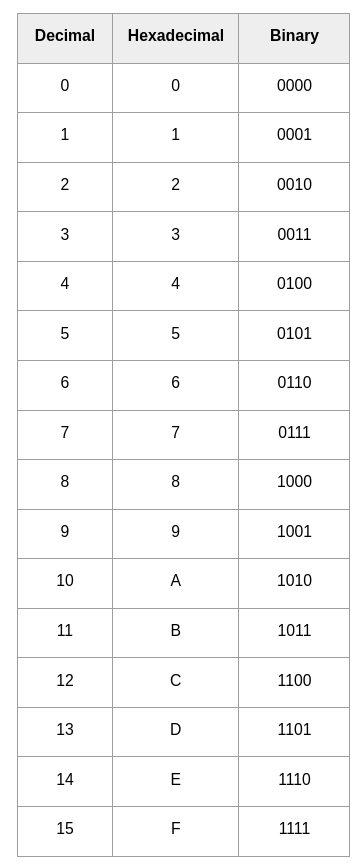
\includegraphics[width=5.0cm]{hex-chart.png}
		\end{center}
	
		\par\noindent \textbf{(II)} We'll denote hexadecimals, binary numbers, and decimals with the subscripts 16, 2, and 10 respectively. So let's figure out what \( (F4A)_{16} \) is in decimal. Going from right to left, A is in position 0, 4 is in position 1, and F is in position 2, so:
		
		\begin{flalign*}
			(15)(16)^2 + (4)(16)^1 + (10)(16)^0 = 3,914 \\
			\text{so ...} (F4A)_{16} = (3,914)_{10}
		\end{flalign*} 
	
		
		
	\end{minipage}	
	\hspace{0.45cm}
	\begin{minipage}[t]{.5\linewidth} 
		\par\noindent \textbf{(III)} We can take a decimal number and transform it into a hexadecimal by continuously dividing by 16 and recording the remainder. Let's convert \( (117)_{10}\) into a hexadecimal:
		
		\begin{flalign*} 
			\intlongdivision{117}{16} \;\; \intlongdivision{7}{16}
		\end{flalign*}
		
		\par\noindent We get a remainder sequence of 5 followed by 7, the hexadecimal is the reverse of this sequence so \((117)_{10} = (75)_{16}\).
		\newline
		\par\noindent We can always check this result by converting \((75)_{16}\) to decimal:
		\begin{flalign*}
			(7)(16)^1 + (5)(16)^0 = 117
		\end{flalign*}
		\par\noindent \textbf{(IV)} Let's try to convert \((17,319)_{10}\) into a hexadecimal:  
		\begin{flalign*}
			\intlongdivision{17319}{16} \intlongdivision{1082}{16} \intlongdivision{67}{16}
			\intlongdivision{4}{16}
		\end{flalign*}
		\par\noindent The remainder sequence of 7,10,3,4 is reversed (remembering that the symbol for 10 is A) to get 43A7, so:
		\begin{flalign*}
			(17,319)_{10} = (43A7)_{16}
		\end{flalign*}
		\par\noindent Just like before we can verify this solution:
		\begin{flalign*}
			(4)(16)^3 + (3)(16)^2 + (10)(16)^1 + (7)(16)^0 \\ = 17,319
		\end{flalign*}
	\end{minipage}

\end{document}